\documentclass[10pt]{beamer}

\usetheme[progressbar=frametitle]{metropolis}
\usepackage{appendixnumberbeamer}
\usepackage{lipsum}
\usepackage{amsmath}
\usepackage{amssymb}
\usepackage{booktabs}
\usepackage[scale=2]{ccicons}
\usepackage{pgfplots}
\usepgfplotslibrary{dateplot}
\usepackage{dirtytalk}
\usepackage{xspace}
\newcommand{\themename}{\textbf{\textsc{metropolis}}\xspace}
\definecolor{mpigreen}{HTML}{007977}
\setbeamercolor{frametitle}{bg=mpigreen}
%https://www.overleaf.com/project/60692a72c2db80145723d37f
\title{Exploring Diseases Dataset \\for Chatbot Dialogue Management}

\author{Tai Ng. (Applied Scientist)}

\institute{VINBRAIN INTERNSHIP PROGRAM 2021 }
\titlegraphic{\hfill
\includegraphics[height=3cm]{logo.png}}

\begin{document}


\maketitle

\begin{frame}{Abstract}
	\section{Task-Oriented Dialogue Systems}
	\begin{itemize}
		\item Help users achieve their specific goals.
		\item User forgets some information.
		\item Focus on understanding users, tracking states, and
		generating next actions.
		\item Minimize the number of turns: fewer turns the better.
	\end{itemize}
	
\end{frame}


%\begin{frame}{Introduce Task Dialogue Systems}
%\section{Characteristics}
%A task-oriented dialogue system is developed to perform a clearly defined task. %Usually, the task involves finding information within a database and returning it %to the user, performing an action, or retrieving information from its users.
%\end{frame}

%\begin{frame}{Task Dialogue Systems}
%\section{Technologies}
%Usually, the user’s input is processed by a natural language understanding (NLU) %unit, which extracts the slots and their values from the utterance and identifies %corresponding the dialogue act. This information is passed to the dialogue state %tracker (DST), which infers the current state of the dialogue. Finally the output %of the dialogue manager is passed to a natural language generation (NLG) component.
%\end{frame}

%\begin{frame}{Introduce Task Dialogue Systems}
%\section{Dialogue Management (DM)}

%The DM could be connected to some external Knowledge Base (KB) or Data Base (DB), such that it can produce more meaningful answers.

%The Dialogue Manager consists the following two components: 
%\begin{itemize}
%\item The Dialogue State Tracker 
%\item Policy Learning
%\end{itemize}
%\end{frame}

%\begin{frame}{Introduce Task Dialogue Systems}
%\section{Approach Dialogue Management}
%\begin{itemize}
%\item Rule-based: Finite state machine 
%\item Learning-based: Deep Q-Learning
%\end{itemize}
%\end{frame}

%\begin{frame}{Introduce Task Dialogue Systems}
%\section{Evaluation}
%Two main aspects are evaluated, which have been shown to define the quality of the %dialogue:
%\begin{itemize}
%    \item Task-success
%    \item Dialogue efficiency
%\end{itemize}
%
%\end{frame}

\begin{frame}{Experiments}
\section{Diseases Dataset}
A dataset to provide the students a source to create a healthcare related system.

\begin{figure}[H]
    \centering
    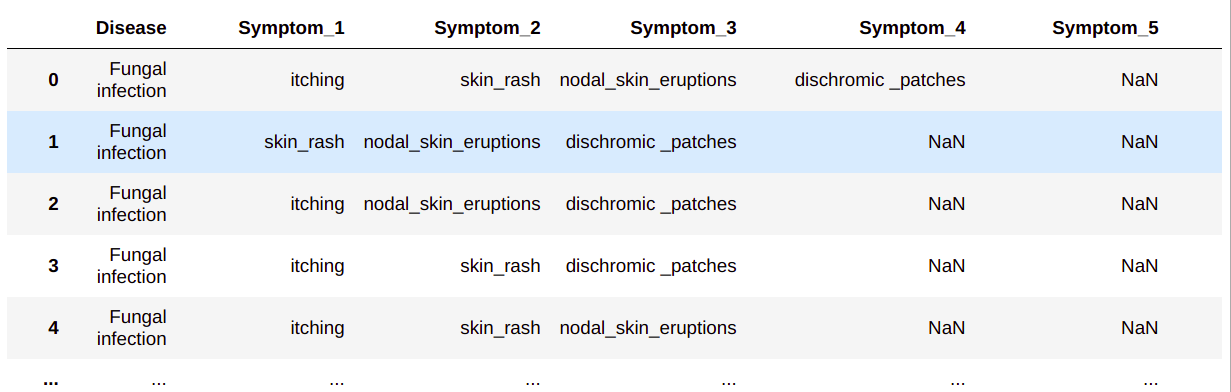
\includegraphics[width=10cm]{image/diseases_dataset.png}
    \caption{Diseases Dataset}
    \label{fig:di_ds}
\end{figure}

\end{frame}

\begin{frame}{Experiments}
    \section{Insight}
    \begin{itemize}
    	\item Dataset has 4920 rows, but it has 41 distinct diseases.
    	\item Synthesizing from multiple sources, symptoms are overlap.
    \end{itemize}
	$\rightarrow$ Re-architecting dataset
\end{frame}


\begin{frame}{Experiments}
    \section{Database}
    \begin{figure}[H]
    \centering
    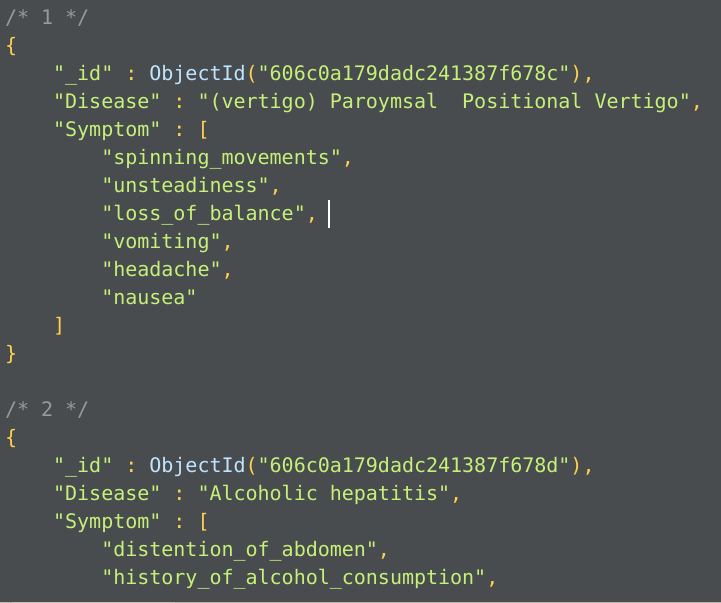
\includegraphics[width=5cm]{image/dbms.png}
    \caption{Disease database}
    \label{fig:di_dbms}
    \end{figure}
\end{frame}

\begin{frame}{Experiments}
    \section{Heuristic}
    \begin{center}
    	\href{https://1drv.ms/u/s!AvgPPwEWTrewcyU0vohmLsytm_4?e=tFHl7o}{Heuristic Search Method}
   	\end{center}
	
\end{frame}



\begin{frame}{Experiments}
    \section{Agent's Action}
    \begin{enumerate}
        \item Inform \& Request: Amount of records greater than one.
        \item Match found: Only one record satisfy user's constraints.
        \item Done: End conversation if cannot found disease.
    \end{enumerate}
\end{frame}

%\begin{frame}{Experiments}
%    \section{Deploy API}
%    \begin{figure}[H]
%    \centering
%    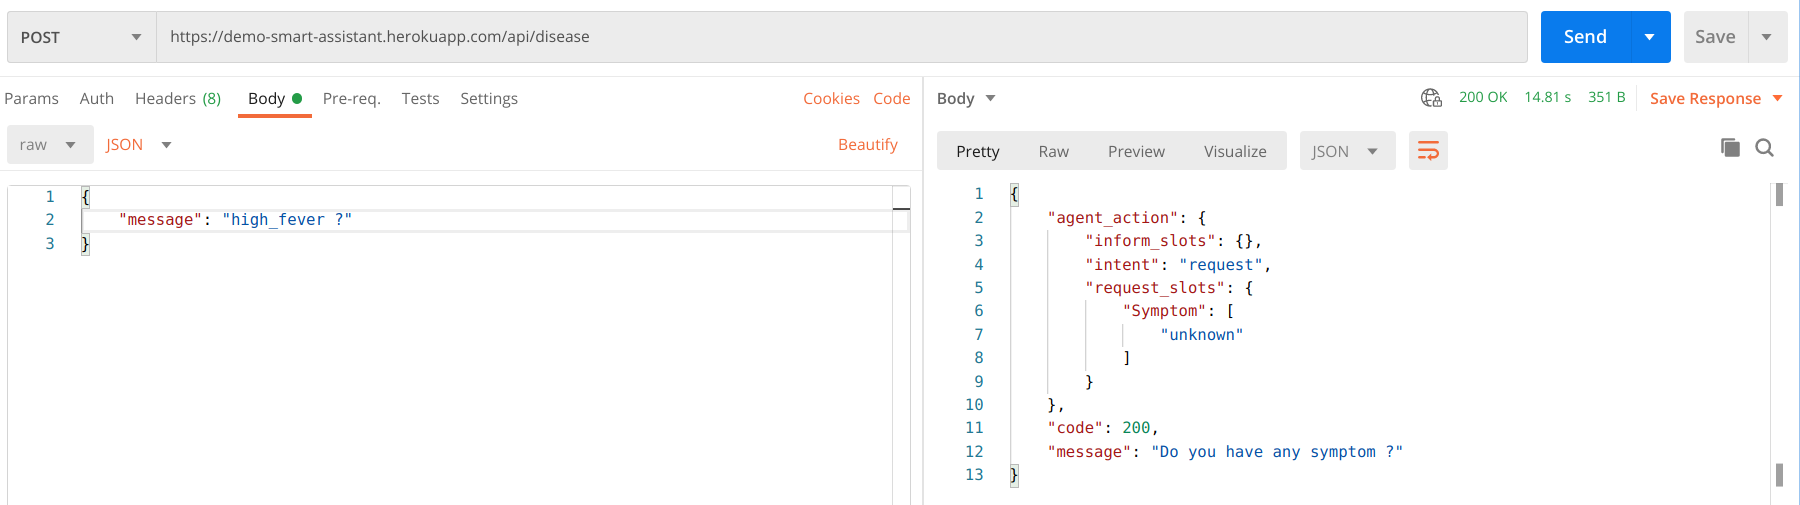
\includegraphics[width=10cm]{image/call_api.png}
%    \caption{API}
%    \label{fig:api}
%    \end{figure}
%\end{frame}

\begin{frame}{Experiments}
    \section{Conversation}
    \begin{figure}[H]
    \centering
    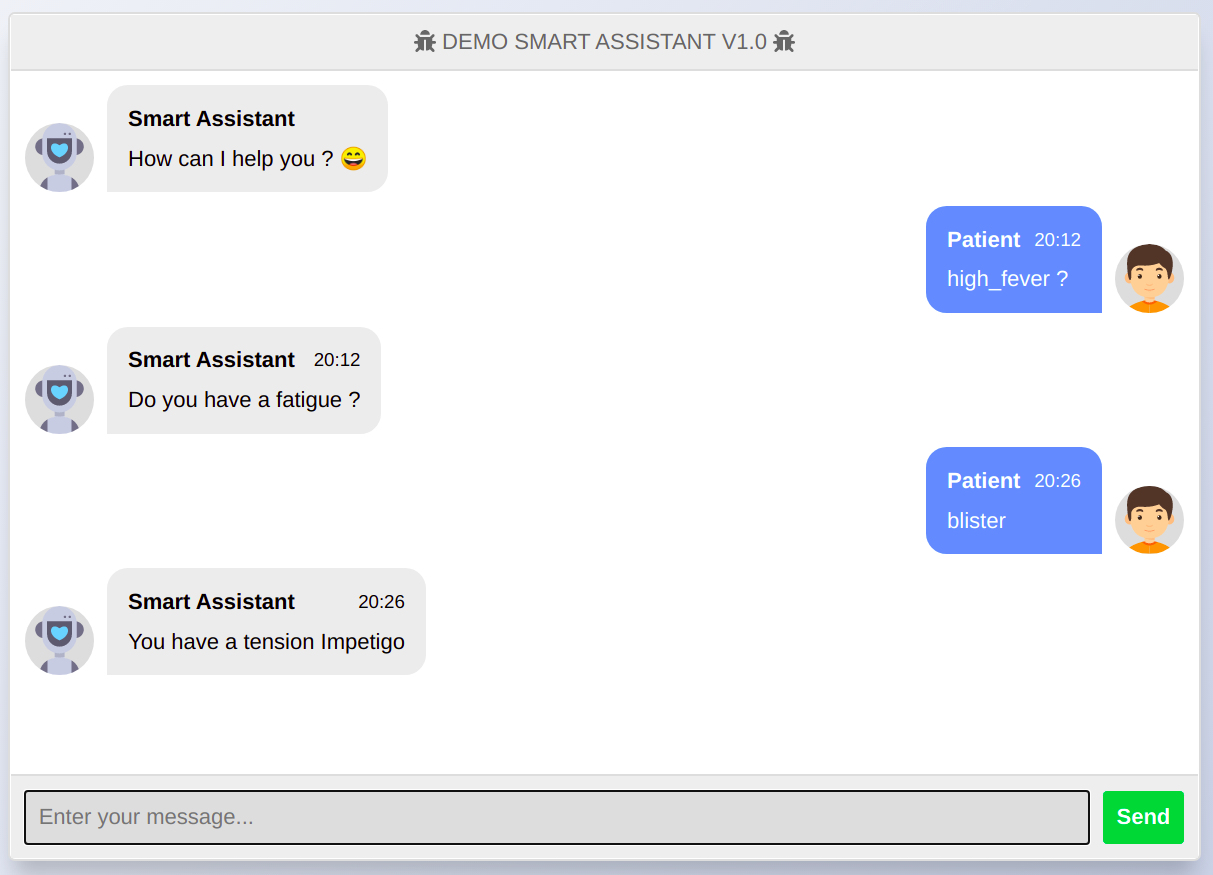
\includegraphics[width=7cm]{image/demo_ui.png}
    \caption{Demo conversation}
    \label{fig:demo}
    \end{figure}
\end{frame}

\begin{frame}{Experiments}
	\section{User's Semantic Frame}
	\begin{figure}[H]
		\centering
		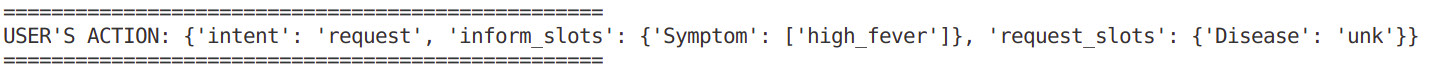
\includegraphics[width=10cm]{image/user_semantic_frame.png}
		\caption{Generate semantic frame from user's action}
		\label{fig:useraction}
	\end{figure}
\end{frame}

\begin{frame}{Experiments}
	\section{Ranking Symptoms}
	\begin{figure}[H]
		\centering
		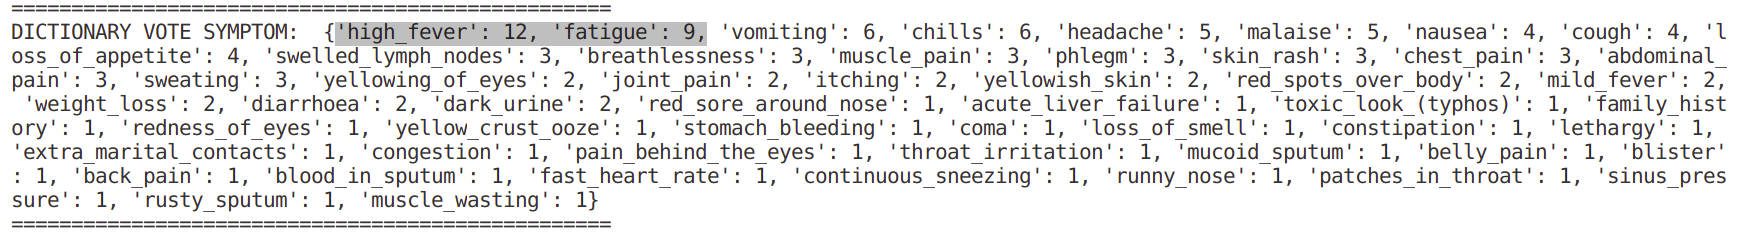
\includegraphics[width=10cm]{image/dict_vote_sympt.png}
		\caption{Count frequency of symptoms in query diseases}
		\label{fig:dict_vote_sympt}
	\end{figure}
\end{frame}

\begin{frame}{Conclusion}
    \begin{center}
        Q\&A
    \end{center}
\end{frame}

\end{document}
